\pagenumbering{arabic}
\section{协议内容声明}

\subsection{自定消息类型}
在本程序中,我们自定消息类型,并将其作为客户端和服务器之间交互信息的载体。我们所定消息的定义如下:

\begin{figure}[H]
  \centering
  % Requires \usepackage{graphicx}
  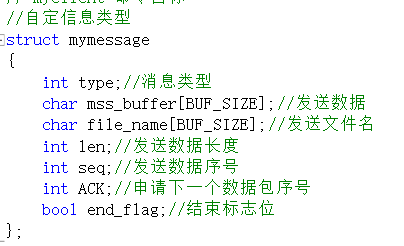
\includegraphics[width=0.8\linewidth]{figure/mymessage}\\
  \caption{mymessage}
\end{figure}

此结构体定义分别被写在myclient类中以及myserver中,从而保证两端信息定义的一致性。在mymessage中,我们分别存放了数据信息,用来发送数据,以及一些必要的标记信息,用来客户端与服务器的交互。
\subsection{自定协议交互过程}

在本次实验中,我们使用一下宏定义信息作为mymessage的type位,用来标记发送信息的类型
\begin{figure}[H]
  \centering
  % Requires \usepackage{graphicx}
  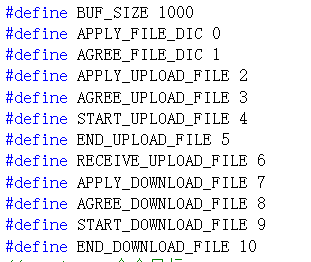
\includegraphics[width=0.8\linewidth]{figure/type}\\
  \caption{mymessage的type位信息}
\end{figure}

协议交互过程如下:

\begin{flushleft}
1)当用户点击获取共享目录时,客户端则会向服务器端发送一个type为APPLY\_FILE\_DIC的消息,服务器端收到此消息后则会回复一个type为AGREE\_FILE\_DIC的消息,并将服务器端的共享目录下的文件加载到发送信息中。\\

2)当用户在客户端选择好要上传的文件并点击开始上传之后,客户端便向服务器发送一条type为APPLY\_UPLOAD\_FILE的消息,并将要上传的文件名包含在消息中。服务器端收到此消息后,便在共享目录创建一个对应的文件,然后发送一条type为AGREE\_UPLOAD\_FILE的消息给客户端。然后客户端逐包发送带有seq的消息,并将type设置为START\_UPLOAD\_FILE。服务器端收到后将收到的包的数据写入创建好的文件,并发送带ACK的消息,将type设置为AGREE\_UPLOAD\_FILE。在客户端发送到最后一个数据包时,会将该条消息的结束标志位end\_flag设置为true。服务器端收到这条消息后将创建的文件流关闭,并向客户端回复一条type为END\_UPLOAD\_FILE的消息,客户端收到后,则跳出。\\


3)当用户在共享目录中选择好要下载的文件,并点击开始下载按钮后,客户端便向服务器端发送一条tpye为APPLY\_DOWNLOAD\_FILE的消息,在这条消息中同样包含了要下载文件的文件名。当服务器端收到这条消息后,则使用文件流打开客户端想要下载的文件,并给客户端打开相应的文件流,回复一条type为AGREE\_DOWNLOAD\_FILE的消息,并把此消息的seq置为-1。而当客户端收到type 未AGREE\_DOWNLOAD\_FILE的消息后,客户端便开始下载工作。每次发送一条type为START\_DOWNLOAD\_FILE的消息给服务器端,客户端收到后回复相应的数据包,客户端收到后将其写入打开的文件流,最后结束后将文件流关闭(此过程与上传过程基本一致)。



\end{flushleft}

\clearpage






























